	\documentclass[11pt,a4paper]{article}
\usepackage[utf8]{inputenc}
\usepackage{amsmath}
\usepackage{amsfonts}
\usepackage{graphicx}
\usepackage[table,xcdraw]{xcolor}

\DeclareUnicodeCharacter{00A0}{ } %este rollo es para evitar un error por la aparición de un caracter invisible e hijo de puta

\usepackage{caption}
\usepackage{subcaption}

\renewcommand{\familydefault}{\sfdefault} % cambiamos la fuente a una sans

\usepackage{float} % para que floten las imagenes o algo asi...
\usepackage{wallpaper} %paquete para usar una imagen como encabezado!
\usepackage{hyperref} %para usar hypervinculos 
\usepackage[export]{adjustbox} %para usar marcos en imagenes
\usepackage{eurosym} % para el euro
\usepackage{transparent} %para las marcas de agua
\usepackage{eso-pic}  %para las marcas de agua

\definecolor{azul_marcos}{RGB}{0,128,159} %defino el color azul de los marcos
\usepackage{sectsty} %esto es para cambiar el color de las fuentes creo
\renewcommand{\familydefault}{\sfdefault} % cambiamos la fuente a una sans
\sectionfont{\color{azul_marcos}}  % sets colour of sections
\subsectionfont{\color{azul_marcos}}  % sets colour of sections


\usepackage{pdfpages} %para insertar pdfs
\usepackage{amssymb}
\usepackage{pstcol} % para color
\usepackage{pst-node} % para diagramas
\usepackage{pst-plot} % para representacion de dat
\usepackage[spanish]{babel}
\addto\captionsspanish{\renewcommand\chaptername{Bloque}}
%\usepackage[total={18cm,21cm},top=2cm, left=2cm]{geometry}
\usepackage{anysize}
\pagestyle{plain}
%\markboth{left head}{right head}
%\markright{Guía de impresión ABS Tech}
\marginsize{3cm}{2cm}{2.5cm}{1cm}
\title{Guía de impresión PETG Tech}
\date{}

%configuracion de la marca de agua
\AddToShipoutPicture{
    \put(0,0){
        \parbox[b][\paperheight]{\paperwidth}{%
            \vfill
            \centering
            {\transparent{0.1}
\includegraphics[scale=1.25]{FOTOS/logofff}}%
            \vfill
        }
    }
}

\begin{document}
\ULCornerWallPaper{1}{FOTOS/header}
\LLCornerWallPaper{1}{FOTOS/footer}
%\maketitle
%\tableofcontents

\includepdf{PDF/PORTADA.pdf}
\section{What is the PETG Tech Filament?}PETG Tech is a filament for 3D printing FFF / FDM of polyethylene terephthalate glycol (P.E.T.G.) designed to combine the best of PLA and ABS being so a resistant thermoplastic and easy to print.
\begin{figure}[H]
\centering
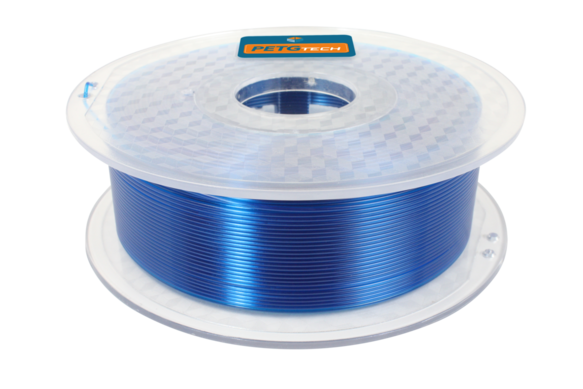
\includegraphics[width=0.5\textwidth,cfbox=azul_marcos 1pt 0pt]{FOTOS/PETGKILOAZUL}
\end{figure}
\section{Why should you use the filament PETG 3D Tech?}PETG Tech is one of the most versatile filaments of the market because it combines the best properties of other materials.
\begin{itemize}
\item PETG is very resistant, almost as much as ABS, so it can be used to construct parts that are going to suffer mechanical stress by traction, pressure or the impact.
\item The PETG also withstands the temperature better than PLA and it has a good resistance to chemicals and also the solvents. It also withstands the UV exposure better than PLA and ABS.
\item It also withstands the UV exposure better than PLA and ABS.
\item In addition PETG filament shows much less "warping" (or tendency to deform when cooling) than ABS and, with the right methods, it can be completely controlled. Therefore this is why PETG filament, in contrast to the others, it allows the printing of large volumes in home printers.
\item Being a less hygroscopic material it is also better and more easily preserved than the PLA.
\item Although the PETG filament is not certified to be in contact with food (FDA Food Safety) the pellet from which it is made does have it and this makes it more suitable for possible contact with food than other materials.Later we analyze in depth this aspect.
\item The PETG is naturally translucent and shiny. Although it is also sold in opaque colors they retain a shiny finish.
\item PETG is a recyclable and biodegradable material just like PLA.
\end{itemize}
Below is a comparative table between the PETG the PLA and the ABS:
\begin{table}[H]
\centering
\begin{tabular}{l|c|c|c|}
\cline{2-4}
                                                                                      & \cellcolor[HTML]{FFFFFF}PLA & \cellcolor[HTML]{FFFFFF}ABS & \cellcolor[HTML]{FFFFFF}PETG \\ \hline
\rowcolor[HTML]{FFFFFF} 
\multicolumn{1}{|l|}{\cellcolor[HTML]{FFFFFF}High impact resistante}          &                             & X                           & X                            \\ \hline
\rowcolor[HTML]{FFFFFF} 
\multicolumn{1}{|l|}{\cellcolor[HTML]{FFFFFF}Low deformation on cooling (warping)} & X                           &                             & X                            \\ \hline
\rowcolor[HTML]{FFFFFF} 
\multicolumn{1}{|l|}{\cellcolor[HTML]{FFFFFF}Absorbs low moisture}                    &                             & X                           & X                            \\ \hline
\rowcolor[HTML]{FFFFFF} 
\multicolumn{1}{|l|}{\cellcolor[HTML]{FFFFFF}Biodegradable}                           & X                           &                             & X                            \\ \hline
\rowcolor[HTML]{FFFFFF} 
\multicolumn{1}{|l|}{\cellcolor[HTML]{FFFFFF}FDA Food safety *}                       &                             &                             & X                            \\ \hline
\rowcolor[HTML]{FFFFFF} 
\multicolumn{1}{|l|}{\cellcolor[HTML]{FFFFFF}Good resistance to the UV rays}            &                             &                             & X                            \\ \hline
\rowcolor[HTML]{FFFFFF} 
\multicolumn{1}{|l|}{\cellcolor[HTML]{FFFFFF}No odor when it is printed}                 & X                           &                             & X                            \\ \hline
\end{tabular}
\end{table}
\section{Technical data and the printing parameters}
\begin{table}[H]
\centering
\caption*{Data sheet}
\begin{tabular}{|
>{\columncolor[HTML]{FFFFFF}}l |
>{\columncolor[HTML]{FFFFFF}}c |}
\hline
\multicolumn{1}{|c|}{\cellcolor[HTML]{FFFFFF}\textbf{Material}}   & Polyethylene glycol terephthalate\\ \hline
\textbf{Available colors}              & 5 (3 translucent, 2 opaque)                 \\ \hline
\textbf{Available formats}             & 1kg, 250gr         \\ \hline
\textbf{Thermal deflection temperature} & 70               \\ \hline
\textbf{Melting temperature}            & 200ºC              \\ \hline
\textbf{Decomposition temperature}    & \textgreater 280ºC \\ \hline
\textbf{Density}                         & 1.27 gr / cm3      \\ \hline
\textbf{Impact resistence}                         & 100 kg-cm / cm      \\ \hline
\textbf{Maximum Stretch}              & 140\%              \\ \hline
\end{tabular}
\end{table}

%TABLA PARAMETROS IMPRESION MEDIA

\begin{table}[H]
\centering
\caption*{Parameters for average printing}
\begin{tabular}{|
>{\columncolor[HTML]{FFFFFF}}l |
>{\columncolor[HTML]{FFFFFF}}c |}
\hline
\multicolumn{1}{|c|}{\cellcolor[HTML]{FFFFFF}\textbf{Recommended Printing Temperature}} & 245º              \\ \hline
\textbf{Recommended printing speed}                         & 55 mm/s              \\ \hline
\textbf{Layer height}                                  &  0.2 mm        \\ \hline
\textbf{Heated bed temperature}                                  &  70º - 85º        \\ \hline
\textbf{Layer fan}                                  &  75\%        \\ \hline
\textbf{Extrusion multiplier **}                                  &  85\% / 100\%        \\ \hline

\textbf{Retraction}                                      & Normal o increased                 \\ \hline
\end{tabular}
\end{table}

%TABLA PARAMETROS RESISTENCIA

\begin{table}[H]
\centering
\caption*{Recommended printing parameters for maximum strength and less transparency *}
\begin{tabular}{|
>{\columncolor[HTML]{FFFFFF}}l |
>{\columncolor[HTML]{FFFFFF}}c |}
\hline
\multicolumn{1}{|c|}{\cellcolor[HTML]{FFFFFF}\textbf{Recommended Printing Temperature}} & 260º              \\ \hline
\textbf{Recommended printing speed}                         & 40 mm/s              \\ \hline
\textbf{Layer height}                                  &  0.2 mm        \\ \hline
\textbf{Heated bed temperature}                                  &  70º - 85º        \\ \hline
\textbf{Layer fan}                                  &  Off        \\ \hline
\textbf{Extrusion multiplier **}                                  &  85\% / 100\%        \\ \hline

\textbf{Retraction}                                      & Normal o increased                 \\ \hline
\end{tabular}
\end{table}

%TABLA PARAMETROS TRANSPARENCIA

\begin{table}[H]
\centering
\caption*{Recommended printing parameters for maximum transparency * and less resistance}
\begin{tabular}{|
>{\columncolor[HTML]{FFFFFF}}l |
>{\columncolor[HTML]{FFFFFF}}c |}
\hline
\multicolumn{1}{|c|}{\cellcolor[HTML]{FFFFFF}\textbf{Recommended Printing Temperature}} & 235º - 240º             \\ \hline
\textbf{Recommended printing speed}                         & 70mm/s              \\ \hline
\textbf{Layer height}                                  &  0.3 mm        \\ \hline

\textbf{Layer fan}                                  &  100\%        \\ \hline
\textbf{Number of perimeters}                                  &  1        \\ \hline
\textbf{Infill}                                  &  0\%        \\ \hline
\textbf{Heated bed temperature}                                  &  70º - 85º        \\ \hline
\textbf{Extrusion multiplier **}                                  &  85\% / 100\%        \\ \hline

\textbf{Retraction}                                      & Normal o increased                 \\ \hline
\end{tabular}
\end{table}
* Only crystalline finishes can be expected in hollow pieces with a single perimeter, ideally glass-like objects.\\\\
** In some printers it may be necessary to reduce the multiplier extrusion. If you see an excess of material in the printed piece in the form of small plastic balls or note that the nozzle collides with the workpiece during printing, then reduce the multiplier extrusion 85\% and gradually increase it until you find the point where the extrusion is appropriate.\\\\
*** If you have stringing problems then try increasing the speed and the distance of retraction. You can download our complete printing profiles of the main programs (Cura, Slic3r and SImplify3D) from our website:
\\\\
\centerline{ {\huge \url{www.fffworld.com/documentation} } }
\\\\
The optimal parameters will depend on the 3D printer you use, however, these are good parameters to have them as a starting point. With a few impressions you will be able to find the limits and the perfect setting for your machine.
\section{PETG Tech: The Characteristics and the printing tips}
	\subsection{The resistance of PETG}PETG can be used to make extremely resistant parts.
\\\\
The PETG is slightly flexible and this allows it to absorb energy before breaking but what really makes the difference with other materials is the consistency of the bond between layers that this material provides.
\begin{figure}[H]
\centering
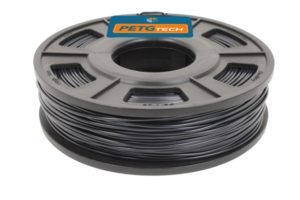
\includegraphics[width=0.5\textwidth,cfbox=azul_marcos 1pt 0pt]{FOTOS/PETG250NEGRO}
\end{figure}
The adhesion of the layers is so firm that sometimes the pieces have greater resistance on the traction between the layers than on the longitudinal axis of the extruded filament track.
\\\\
The resistance between the layers can be increased by raising the temperature or decreasing the speed. This allows that the melted material is deposited hotter and in a slower way.
\\\\
However the finish of the piece will be worse and the transparency will be reduced as a result of plastic tracks slightly deformed by the excess temperature. The layer fan here plays in favor of transparency and of the finish product but also toward the overall strength of the piece.
\\\\
Keep in mind the above when laminating, depending on the type of piece and use that you will give.
	\subsection{The transparency of PETG}PETG is a translucent material like the PET which is used in making plastic containers completely transparent. However, it must be taken into account that the manufacturing processes of these containers differ greatly from those used in 3D printing
\begin{figure}[H]
\centering
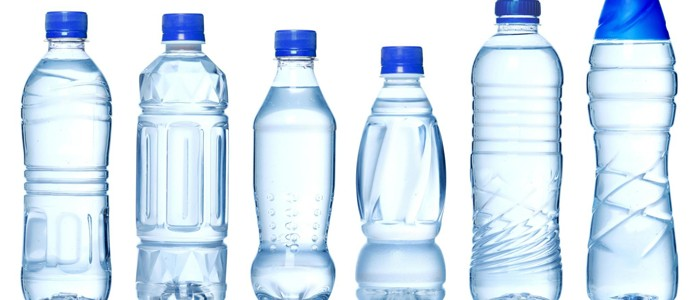
\includegraphics[width=0.5\textwidth,cfbox=azul_marcos 1pt 0pt]{FOTOS/BOTELLASPET}
\end{figure}
 And for that reason to obtain a piece printed in 3D completely crystalline is not possible, at least using technology FFF / FDM.
\\\\
In addition to accumulating horizontal perimeters the increasing of the thickness of the walls of the pieces reduces the transparency. However if your goal is to get translucent pieces we do offer some tricks.
\\\\
As a general rule, the higher the temperature or the lower the speed, then the transparency of the printed part is less. This is because the hot plastic tends to drain creating curved surfaces that deflect the light.
\\\\
With higher speeds and the lower temperatures it is possible to ensure that the cast plastic tracks are deposited in a more regular way favoring the transparency of the part.
\\\\
	Depending on the axis where you need a more translucent finish, you can also follow the following tips.
		\subsubsection{The transparency in axis Z (vertical)}The transparency of the piece is going to be a function of the height of the piece and the infill used.
\\\\
Also the number of layers so the recommendation is to use a greater layer height to in order to reduce the number of them.
\\\\
We must differentiate between the layers that make up the base of the piece, and which are printed directly on the printing surface, of those that serve as cover or top enclosure.
\\\\
In the first ones the transparency will be good since the molten plastic takes a flat and regular shape when it is deposited on a flat surface.
\\\\
The upper ones, however, tend to arch as they rest on the outer horizontal perimeters and the filling structure. This is why the lower layers have better transparency than the upper layers.
\\\\
To diminish this problem you can increase the speed with which the printer extrudes the top layers so that they are tenser and less irregular.
\\\\
This is an advanced option that is not available in all laminated programs.
		\subsubsection{The transparency in XY plane (horizontal)}In the XY plane the way to increase transparency is to reduce the number of perimeters.
\\\\
However if the piece has some kind of infill it will subtract transparency equally so that it is only possible to get pieces with high transparency in pieces those of glass types.
\\\\
For these types of parts the laminating programs offer the option of printing by increasing the Z position continuously when you want to print with a single perimeter. This option is known as to spiralize (Cura), or the vase mode (Slic3r and Simplify) and it is the one we recommend in order to obtain the best results in terms of transparency.
\\\\
As we have already mentioned the higher the speed and the lower the temperature the better the transparency as a consequence of a more regular arrangement and tense the plastic tracks so the tests should be directed to find the maximum speed and the minimum temperature that allows to print pieces without separating the layers .
\\\\
A speed of 70 mm / s with a temperature of 240º and a layer height of 0.25 mm should provide good transparency in pieces printed in (vase mode) although this is dependent on the workpiece and on the machine.
	\subsection{The 3D PETG filament and the food safety (FDA Food Safety) of 3D printed objects}The PETG and the PET are very similar plastics and it is known that the latter is widely used in the manufacture of plastic food containers. This is because both have a certification issued by the FDA that guarantees the health of food coming into contact with such materials.
\begin{figure}[H]
\centering
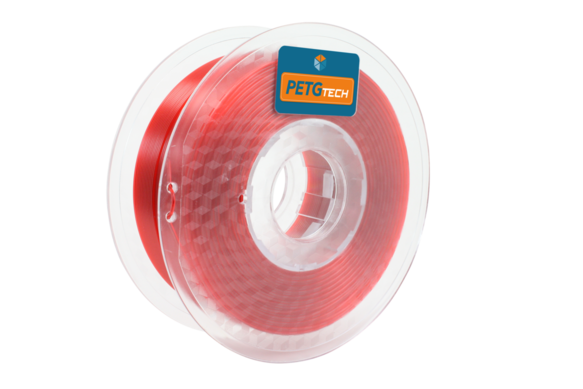
\includegraphics[width=0.5\textwidth,cfbox=azul_marcos 1pt 0pt]{FOTOS/PETGKILOROJO}
\end{figure}
While this is true, it must be understood that the certification refers to the pellet (the raw material) from which the filaments of PETG are produced and that such certification cannot be transposed directly for different reasons that we are going to analyze.
\\\\
First, the 3D printing filaments often contain additives to provide them with characteristics that improve their performance when they are used.
\\\\
The inclusion of any additive that does not have FDA Food Safety certification prevents it from being applied.
\\\\
On the other side most of the filaments are mixed with dyes to give them color and although these dyes are certified ROHS are not FDA Food Safety certified.
\\\\
The first (ROHS) certifies the absence of harmful elements (such as lead or mercury), while the second certifies the absolute safety of the certified object to the extent that it may be in contact for a long time with food intended for consumption.
\\\\
Therefore the mere addition of non-FDA Food Safety colors prevents its consideration as such.
\begin{figure}[H]
\centering
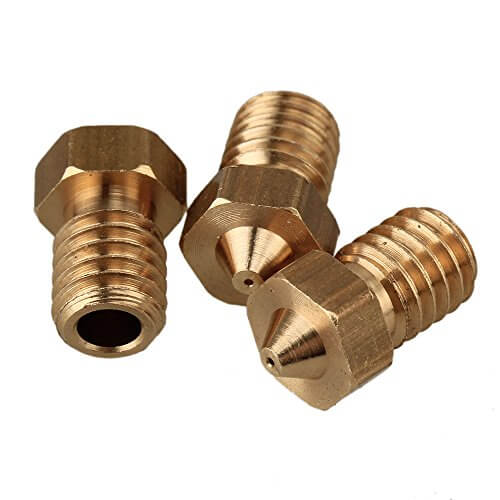
\includegraphics[width=0.5\textwidth,cfbox=azul_marcos 1pt 0pt]{FOTOS/NOZZLES}
\caption*{The nozzle may contain lead}
\end{figure}
Even in the case of filaments whose base material, additives and dyes are FDA Food Safety certified, the process of printing on a domestic machine prevents the resulting object from being certified.
\\\\
This is a consequence of the metals with which the nozzle (brass) and the extruder that pushes the filament are made of.
\\\\
For all of the above it is not possible to create objects using FFF 3D printing that comply with FDA Food Safety. With all the above, it is necessary to establish the difference between special and general food safety.
\\\\
The first is granted by agencies such as the FDA, that guarantees the health and are obliged to offer certain guidelines in their products.
\\\\
The second, the general food security, is the confidence that anyone can have, based on their reason and experience, that a particular food does not contain any harmful element after its manipulation.
\\\\
While 3D-printed objects cannot be FDA-certified, it is safe to assume that nobody can become intoxicated by eating a cookie that has been cut with a 3D-printed cookie mold or by using a glass or a disposable 3D printed cover.
\begin{figure}[H]
\centering
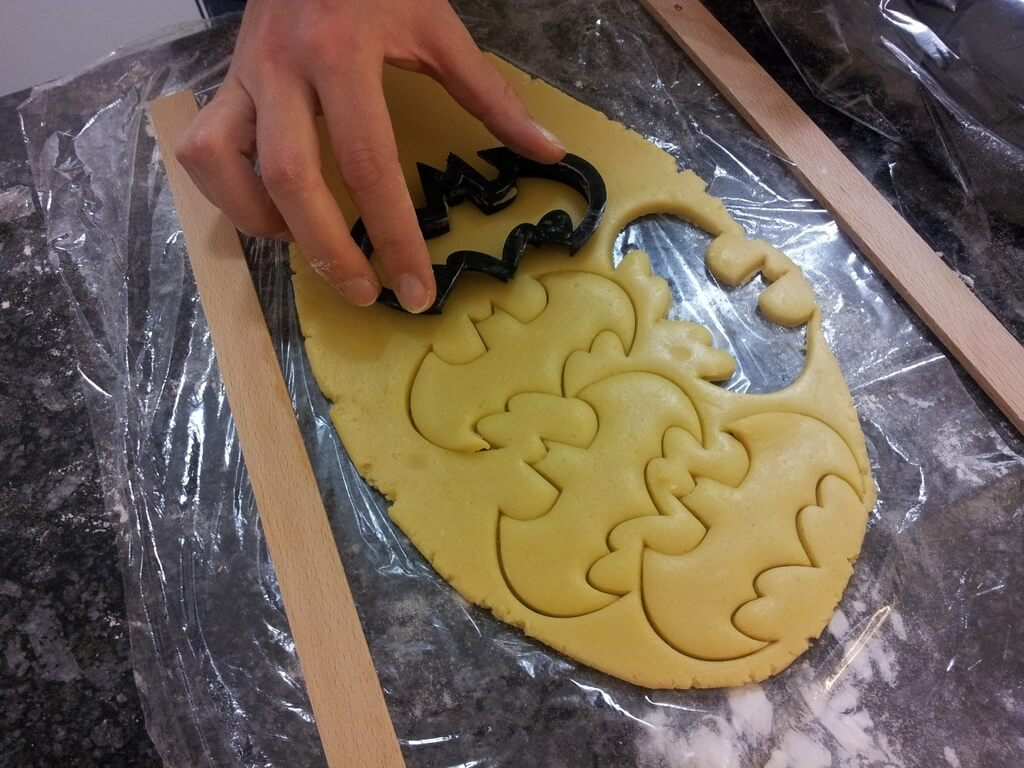
\includegraphics[width=0.5\textwidth,cfbox=azul_marcos 1pt 0pt]{FOTOS/CORTADORGALLETAS}
\end{figure}
Now you have to take into account some things when it comes to printing objects that are going to be in contact with food:
\begin{itemize}
	\item 3D FFF / FDM printing tends to leave small spaces and interstices on the surface of the pieces that favor the development of bacteria and microorganisms. If the piece is to be of single use it may not be a problem but if it is to be reused consider applying a Food Safety epoxy coating to seal the surface of the piece.
	\item Such organisms should die when using a dishwasher because of the high temperature of the water but such temperature can deform the part.
	\item The contact time between the food and the piece is important; a bottle is not the same as a fork or a cookie cutter.
\end{itemize}
\section{The problems and solutions when printing 3D filaments PETG}
	\subsection{How to correctly attach the PETG to the printing surface}The PETG has less warping than the ABS and it can be controlled, however it is necessary that the first layer is perfectly glued to the printing surface in order to print in a satisfactory way.
\\\\
The best method is to use warm bed at 75º and to print on the glass by applying standard lacquer. In case there is no hot bed it is recommended to use the brim option of the laminate program and to lower the speed of the first layer so that it is firmly adhered to the printing surface.
\begin{figure}[H]
\centering
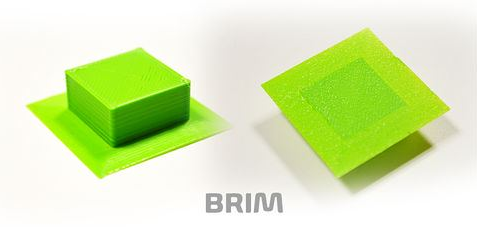
\includegraphics[width=0.5\textwidth,cfbox=azul_marcos 1pt 0pt]{FOTOS/BRIM}
\end{figure}
Problems have been observed when trying to print PETG 3D filaments on blue tape (3M blue tape) or body tape so we recommend using the first method described: lacquer, glass and bed a at 75º
	\subsection{The support structures in PETG}We have already talked about how strong is the bond between the layers of molten PETG, however this presents a challenge when printing pieces that make intensive use of supports.
\\\\
PETG supports are retired with greater difficulty and the finish of the surface in direct contact with the support is rough and irregular.
\\\\
The most advanced lamination programs allow you to configure the horizontal and vertical distance between the part and the supports, as well as the infill and the geometry of the support structures
\\\\
It is recommended to increase these distances, reduce the infill of the support and to opt for a simple geometry of lines if you are having any of the problems mentioned above when using support structures in your parts.
	\subsection{Stringing Problems}The ability of PETG to stick strongly makes it prone to leave debris in the form of threads in the printed pieces.
\begin{figure}[H]
\centering
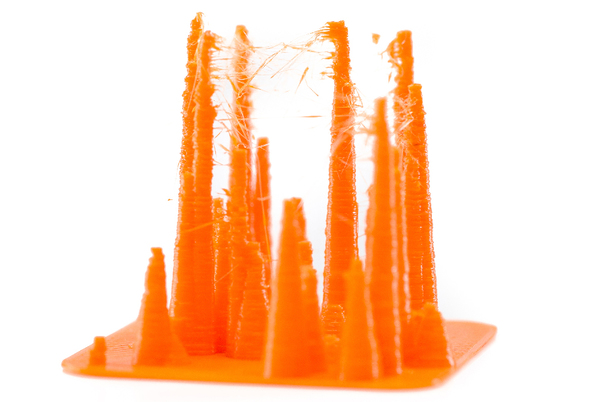
\includegraphics[width=0.5\textwidth,cfbox=azul_marcos 1pt 0pt]{FOTOS/RETRACCION1}
\caption*{Part with stringing problems}
\end{figure}
Besides, when several parts are going to be printed at the same time, these little threads can appear between the parts since the nozzle has to constantly jump from one to others.
\\\\
As we’ve already previously commented this effect can be reduced by using retraction, but it’s highly recommendable that also the different parts be printed sequentially instead of simultaneously.
\\\\
By sequential printing we mean completely printing a part before starting printing the next.
\\\\
This can be achieved in two different ways:
\begin{itemize}
\item The trivial option is to print only one part and once finished repeat the same print as many times as wanted.
\item The second alternative, more advanced and with some limitations, is to use the laminating option that some programs offer instead of printing one part at a time. The maximum size of the parts that can be printed using this method comes given by the dimensions of the nozzle and the disposition of the axis of the printer. We highly recommend that you get information about how to use the options as not to run the risk of damaging your printer. You can do it through the following links:
\end{itemize}
\url{https://www.simplify3d.com/support/tutorials/multi-part-printing/}\\
\url{http://manual.slic3r.org/advanced/sequential-printing}\\
\url{https://ultimaker.com/en/community/3843-force-cura-to-print-objects-separately}
\begin{figure}[H]
\centering
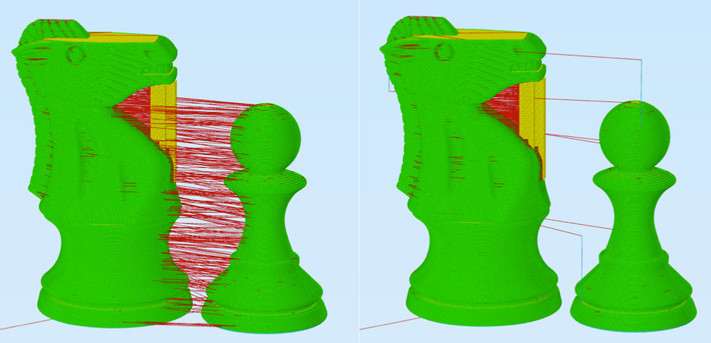
\includegraphics[width=0.5\textwidth,cfbox=azul_marcos 4pt 0pt]{FOTOS/SEQUENTIALPRINTING}
\caption*{Comparison the printing routes betweeng simultaneous and sequential printing}
\end{figure}
\section{Would you like to support our project?}
All the members of FFF World love 3D printing and the maker community. We feel lucky to be able to work on projects where we can deliver our honest passion. In the future, we would like to be able to develop more materials, more colors and more formats. Ultimately, we would like to be able to make our company grow.
\\\\
Therefore, one of the best actions to help us, if you want to do it and you’re satisfied with the filament, is to give us a 5 stars rating on amazon.
\begin{figure}[H]
\centering

\includegraphics[width=0.5\textwidth,cfbox=azul_marcos 1pt 0pt]{FOTOS/AMAZON_FIVE_STARS}
\caption*{Thanks a lot!}
\end{figure}
\subsection{Other filaments with awesome properties available today in Amazon}
\begin{description}
\item[FlexiSMART Tech:] Designed to resist the abrasion and wear of technical printings.
\item[ABS Tech:] Minimized warping effect. High performance on technical applications.
\item[PETG Tech:] Maximum mechanical resistance. Resistant to contact with water and UV rays. Apt for alimentary use.
\item[FilaMETAL:] PLA with non-abrasive metallic charge that gives a spectacular mechanical finish to your printings.
\item[PC Tech:] Polycarbonates with a high resistance to temperature and excellent mechanic properties.
\item[Nylon Tech:] printable at low temperature. Resistance to bangs with a certain degree of flexibility.
\item[PVA Tech:] Water soluble filament indicated for use as support material. Excellent compatibility with PLA.
\item[HIPS Tech:] Limonene soluble filament indicated for use as support material. Good mechanical resistance and excellent compatibility with ABS.
\end{description}
%\section{Bibliografía}
%Esta guía no habría sido posible sin el conocimiento libre generado por la comunidad RepRap. Para la elaboración de esta guía se han %utilizado imágenes y contenido extraidos de los siguientes sitios web.
%\\\\
%\url{http://www.gyrobot.co.uk/blog/how-to-3d-print-with-flexible-filaments}\\
%\url{http://www.thingiverse.com/thing:1496895}\\
%\url{http://www.thingiverse.com/thing:247024}\\
%\url{http://www.thingiverse.com/thing:16319}\\
%\url{http://www.thingiverse.com/thing:779011}\\
%\url{http://www.thingiverse.com/thing:1102900}\\
%\url{http://www.thingiverse.com/thing:147705}\\
%\url{http://www.thingiverse.com/thing:222667}\\
%\url{http://www.thingiverse.com/thing:512338}\\
%\url{https://all3dp.com/common-3d-printing-problems-and-their-solutions/}\\
%\url{https://www.simplify3d.com/support/}\\
%\url{http://www.thingiverse.com/thing:508896}\\
%\url{http://www.thingiverse.com/thing:1187344}

\includepdf{PDF/EN_CONTRAPORTADA.pdf}
\end{document}
